\section{Input Catalogs and Data Preparation}
\label{sec:data}

Our principal data source is the merged WISE-2MASS catalog. In order to derive
WISE-2MASS color-based selection criteria, we use %several training samples
%described below: a heterogeneous sample of bright \agb\ stars listed in 
%SIMBAD database and more homogneous fainter samples selected using 
%optical time-domain surveys OGLE-III and MACHO. The latter samples 
%include \agb\ stars from the LMC and SMC and are also used to 
%calibrate color-absolute magnitude relations that underlie our distance
%estimates. In order to assess what infrared populations could contribute to
%contamination of selected \agb\ candidates, we utilize a number of SDSS
%catalogs, also described below. We conclude this section by describing
%how these catalogs auxiliary catalogs were  positionally merged with the 
%WISE-2MASS catalog and summarize the object counts before and after quality control in Table 1 
a homogenous sample of AGB stars from the OGLE-III Catalog of Variable Stars supplying objects in the Magellanic Clouds. This sample serves to calibrate color-color and color-absolute magnitude
relations that underlie our distance estimates. In order to assess what infrared populations
could contribute to contamination of selected \agb\ candidates, we utilize
extragalactic sources from SDSS data release 7 pulled from the NYU Value-added Galaxy Catalog,
the SDSS unofficial Luminous Red Galaxy sample,
and young stellar objects identified in \wise\ data, also described below. 
We conclude this section by describing how these auxiliary catalogs were positionally merged
with the WISE-2MASS catalog, summarize the object counts before and after quality control (Table~\ref{tab:reductions}), and summarize the effects of WISE-2MASS color-color cuts (Tables~\ref{tab:criteria_completeness} \& ~\ref{tab:criteria_contamination}) on the AGB and contaminant samples. 

\subsection{WISE-2MASS catalog}
In this study, we rely heavily on data from the \allwise\, extension of the \wise\, survey, combining data from the initial All-Sky Data Release, the 3-band cryogenic data release, and the NEOWISE post-cryogenic data release \citep{2013wise.rept....1C}. The initial \wise\,All-Sky Data Release observed the sky between January and August 2010, observing the sky 1.2 times on average with four detectors, operating at 3.4, 4.6, 12, and 22$\mu$m. Hereon we refer to \allwise\, photometric bands at [3.4$\mu$m/4.6$\mu$m/12$\mu$m/22$\mu$m] as [$W1/W2/W3/W4$]. The positions of objects in the \wise\, catalog were calibrated using the \twomass\, point source catalog. 

The 3-band cryogenic data release contains data from $W1$, 2, and 3, and surveyed $30\%$ of the sky between August and October 2010. During the 3-band cryogenic survey, $W1$ and $W2$ operated with nearly the same sensitivity as during the full survey. Warming of the telescope reduced sensitivity in $W3$ and fully saturated $W4$. The NEOWISE post-cryogenic data release contains $W1$ and $W2$ measurements, with sensitivities close to those obtained during the full cryogenic phase. During this phase, \wise\, surveyed $70\%$ of the sky. Data products from the post-cryogenic release included updated instrumental, astrometric, and photometric calibrations and reduction algorithms, resulting in higher signal-to-noise for most sources. The overall number of sources compiled into \allwise\, totals over 747.6 million.

%\subsection{AGB stars from SIMBAD database}
%The SIMBAD database\footnote{\url{http://simbad.u-strasbg.fr/simbad/}} is comprised of astrometry, classifications, and photometry for all types of astronomical objects from a variety of surveys.  Classifications are hierarchical, and are classified with increasing specificity based on the available data, though each star can have multiple classifications. AGB stars have subcategories of C-stars ([C/O] $>$ 1) and S-stars ([C/O] $\sim$ 1). Where subclassification is unclear, the main classification remains as AGB star. OH/IR stars are subsets of peculiar stars that specifically show strong OH maser emission and strong IR emission, identifying them clearly as AGB stars.  Mira-type variables are a subset of variable stars, and are classified based upon their periodicity. Semi-regular variables are not included as they contain an unknown mixture of AGB stars and red supergiants. The sample of AGB stars from SIMBAD was obtained by querying all objects with types classified as C-stars (23,628), S-stars (1,514), AGB stars (4,459), OH/IR stars (1,265), and Mira-type variables (10,828). Without duplicate objects between the five types, there is a total of 39,348 AGB stars from SIMBAD.

%\subsection{AGB stars from optical time-domain surveys}
%Many of the identifications in the SIMBAD catalog are from spectroscopic studies, however many more AGB stars have been found through their characteristic optical periodicity. The \emph{Optical Gravitational Lens Experiment} (OGLE) and the \emph{MAssive Compacy Halo Objects} (MACHO) survey are two time-domain microlensing surveys that have captured and catalogued such variability. In Sections~\ref{sec:macho} and \ref{sec:ogle} we disc.uss the origins of the data from each source and how they were then used for this study

%\subsubsection{MACHO}\label{sec:macho}
%The \emph{MACHO} project \citep{1992ASPC...34..193A,1997ApJ...482...89A} was a two-color optical microlensing survey searching for massive compact halo objects in the Milky Way bulge and the Magellanic Clouds. As a consequence of the time-domain survey, the \emph{MACHO} catalog contains 8 years of observations for several million stars, many of which were observed to be variable. 
%Using Fourier decomposition, \cite{2008PhDT.........6F} identified and classified a population of 46,832 LPVs in the LMC, 3,943 in the SMC {\color{red}[check this]} , and {\color{red}[some other number]} in the Milky Way Bulge with matches to 2MASS. We note that due to high scatter and uncertainty of Galactic objects in period-magnitude space, we only take sequences 1 and 2 (Mira-type variables) for the Milky Way Bulge sample. Each object carries observations in Kron-Cousins $V$ \& $R$, and 2MASS photometry. AGB stars are separated from RGBs by identifying the tip of the RGB ($K_s < 12.3$ in the LMC and $K_s < 12.8$ in the SMC). {\color{red}[some small tidbit about the reduction procedure]}. 

\subsection{AGB stars from the OGLE-III Catalog of Variable Stars}\label{sec:ogle}
The OGLE-III Catalog of Variable Stars (CVS) \citep{2008AcA....58...69U,2009AcA....59..239S,2011AcA....61..217S} is a subset of the overall OGLE-III dataset, containing roughly 10 years of observations in the $V$- and $I$-bands of over 120,000 variable stars, with typically 700-900 data points per star in the $I$-band and about 50 data points per star in $V$-band. With high-precision photometry \citep[$~0.01$ mag][]{2007AcA....57..201S}, these observations saturate at $I = 12.5$ mag, and are limited at the faint end at $I = 20.5$ mag \citep{2001AcA....51..303Z}. The variability of these stars covers a wide range of periodicity ($4 < P < 2000$ days) and amplitudes ($0.005 < A_I < 5.7$ mag).

The OGLE-III CVS is accessible through an online database\footnote{\url{http://ogledb.astrouw.edu.pl/~ogle/CVS/}}, with long-period variables (LPVs) classified by object type, evolutionary status, and spectral type. Object type is based chiefly on variability and luminosity. OGLE Small Amplitude Red Giants (hereon OSARGs) are weakly-variable ($0.005 < A_I < 0.13$ mag), with relatively short periods \citep[$10 < P < 100$ days;][]{2004AcA....54..129S}. Additionally, because these objects are multiperiodic, OSARGs are selected using their period ratios and their distances from established period-luminosity (log$P-L$) sequences from \cite{1999IAUS..191..151W}. For a more detailed description of their selection, see \cite{2007AcA....57..201S}. Mira variables and Semi-Regular Variables (hereon SRVs) are identified using $I$-band amplitudes and $P-W_I$, where $W_I$ is the reddening-free Wesenheit index \citep{2005AcA....55..331S}:
\begin{eqnarray}
W_I &=& I - 1.55(V-I)
\end{eqnarray}

As red giant branch stars (RGBs) can contaminate the same log($P)-L$ space as AGB stars, evolutionary type is distinguished in two ways. Stars above the tip of the RGB ($K_s = 12.05$ mag in LMC; \citealt{2004AcA....54..129S, 2007AcA....57..201S}) are classified as AGBs. Below that threshold, a narrow sequence of stars appears to share the same slope and intercept with AGB stars above the TRGB. Additionally they share similar primary-secondary period ratios as known AGB stars \citep{2005AcA....55..331S}. However, as there is still some contamination by RGBs using period ratios, we reject all OGLE objects below the TRGB.

For individual log$(P)-L$ sequences, spectral type (O-rich or C-rich) is easily seen as separations in log$(P)-L$ space as well as visible-NIR color-color space. The initial classifications are based on spectroscopically-observed stars and were extended more generally to log$(P)-L$ and visible-NIR color-color criteria \citep{2005AcA....55..331S, 2007AcA....57..201S}. This clear separation can be seen in Figure~\ref{fig:oglepmag}.

From the initial OGLE-III sample of 52,976 LPVs, we retain 43,262 after matching to ALLWISE within 3", and ensuring only 1 match to 2MASS as well as all objects needing to be in the LMC. The $I$-band median of OGLE-III LPVs is $\approx14.68$ mag with a standard deviation of 0.72 mag. Out of the entire sample only 13 objects (Miras) fall beyond the 20.5 mag 5$\sigma$ faint limit, and 41 beyond the saturation limit. As such, we expect this to effectively represent the complete sample of oscillating AGB stars in the LMC.

Out of the 43,262 objects matched to ALLWISE within 3", 1,633 are Mira variables, 30,768 are OSARGs, and 10,861 are SRVs. The right side of Figure~\ref{fig:oglepmag} shows color-color plots for OGLE-2MASS colors, with a line at $(J-K_s) = 1.4$ drawn to separate O-rich and C-rich Miras. Out of the total of 457 O-rich Miras, 36 (7.9\%) have $(J-K_s) > 1.4$. Conversely, out of the 1,176 C-rich total Miras, 1,138 (96.8\%) have $(J-K_s) > 1.4$. The distribution of these objects on the sky is summarized in Figure~\ref{fig:oglegalplot}.

\begin{figure}[h]
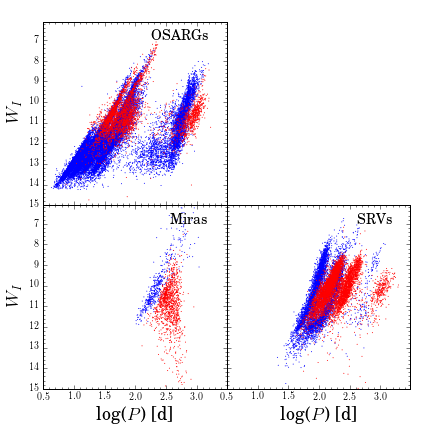
\includegraphics[width=3in]{figs/ogle_2mass_period_mag_threeplot.png}
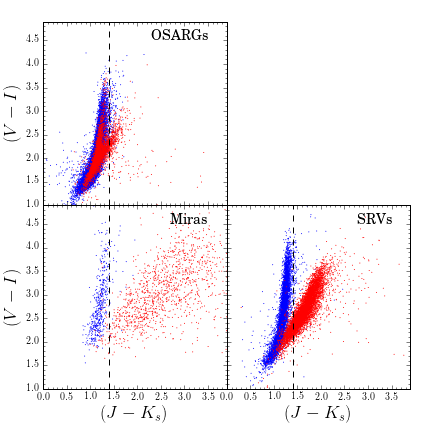
\includegraphics[width=3in]{figs/ogle_2mass_color_color_threeplot.png}
\caption{O-rich (\emph{blue}) and C-rich (\emph{red}) OGLE-III LPVs matched to 2MASS. \emph{Left}: $W_I$ vs log period in days. \emph{Right:} OGLE-III $(V-I)$ vs 2MASS $(J-K_s)$. The dashed line represents $(J-K_s) = 1.4$. \label{fig:oglepmag}}
\end{figure}

\begin{figure}[h]
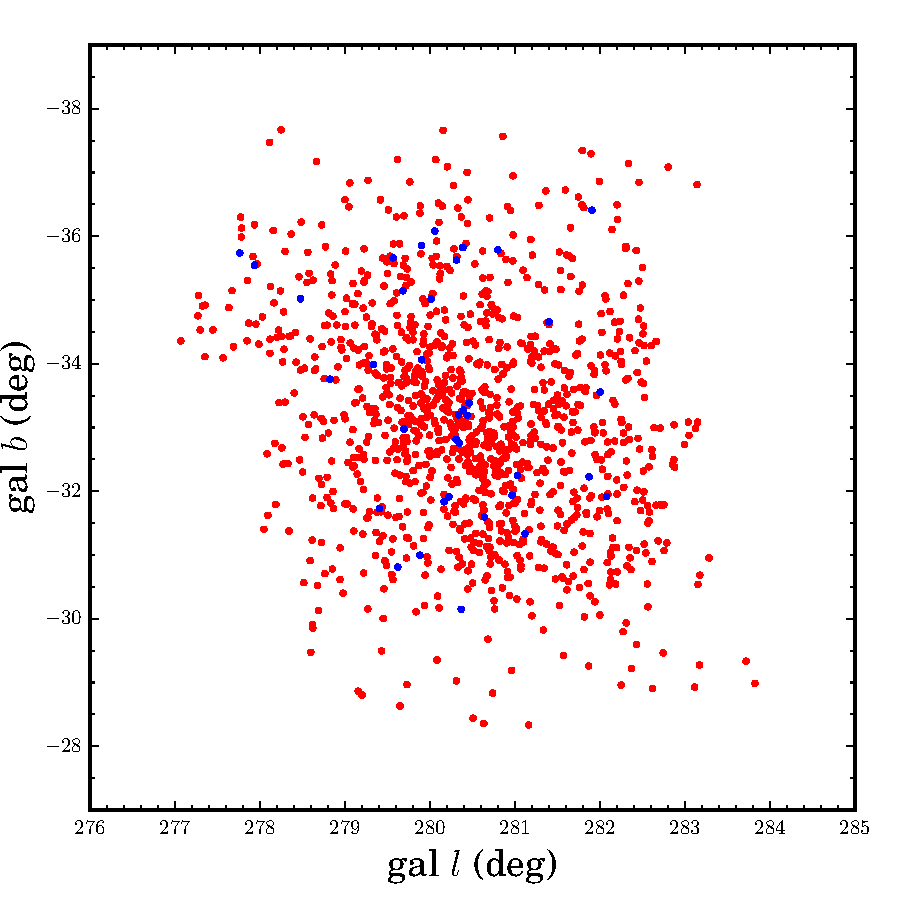
\includegraphics[width=3in]{figs/ogle_2mass_wise_miras.pdf}
\caption{O-rich (\emph{blue}) and C-rich (\emph{red}) OGLE-III Miras with ($J-K_s$) $>$ 1.4. \label{fig:oglegalplot}}
\end{figure}

\subsection{Extragalactic catalogs from SDSS}
SDSS is a multi-year survey of roughly 25\% of the sky that collected both photometric (\emph{u, g, r, i, z}-bands for 700+ million objects) and spectroscopic measurements (1.6+ million) of stars and extragalactic sources \citep{2000AJ....120.1579Y}. Though its ground-based nature and sensitivity to interstellar extinction prevent SDSS from being an all-sky survey, it represents the largest spectrophotometric catalog to date. For this study we collect extragalactic objects from the NYU Value-added Galaxy Catalog, containing objects matched between SDSS and several auxiliary surveys spanning multiple wavelength regimes, and the SDSS Luminous Red Galaxy sample, isolating high-confidence luminous red galaxies from the SDSS database. The color-color distributions of these sample sets are shown in Figure~\ref{fig:wisecontaminants}.

\subsubsection{The NYU Value-added Galaxy Catalog}
In order to cull the full set of SDSS spectrophotometry and produce an easily-referenced extragalactic catalog for investigating galaxy formation and evolution, the NYU Value-added Galaxy Catalog \citep[NYU-VAGC;][]{2005AJ....129.2562B} was created as of SDSS data-release 7 (DR7). 

The NYU-VAGC contains matches between SDSS spectrophotometry and the following catalogs: the FIRST radio survey, the 2MASS Point Source Catalog, the 2MASS Extended Source Catalog, the Two-degree Field Galaxy Redshift Survey, the IRAS Point Source Catalog Redshift Survey, and Reference Catalog 3 (RC3.9b). As a consequence, the NYU-VAGC retains SDSS optical photometry in addition to spectral classifications (QSO, galaxy, star) and subclassifications (AGN, starforming galaxy, starburst galaxy, etc.) for 441,707 objects across 10,417 square degrees of the SDSS footprint. Main and secondary classifications are made by comparing measured optical spectra to the SDSS spectral library. See \cite{2005AJ....129.2562B} for the full set of reduction and inclusion criteria. This catalog is available via an online data repository\footnote{\url{http://sdss.physics.nyu.edu/vagc/}}, along with a full description of the data and other subsamples not used in this study. The populations for each species (QSO, AGN, starforming galaxy (SF), starburst galaxy (SB)) are found in Table~\ref{tab:reductions}.

\subsubsection{The Luminous Red Galaxy Sample}
Subselected for the study of Baryon Acoustic Oscillations by \cite{2010ApJ...710.1444K}, the Luminous Red Galaxy sample \citep[LRGs;][]{2001AJ....122.2267E} is also sourced from SDSS DR7. LRGs contaminate the IR color-color space of AGB stars due to their large redshifts ($z\sim0.3$). We obtain the  LRG sample from the data repository\footnote{\url{http://cosmo.nyu.edu/~eak306/SDSS-LRG.html}} of \cite{2010ApJ...710.1444K}. The initial sample is volume-limited, containing 105,631 objects spanning a redshift range of $0.16 < z < 0.47$.

\begin{figure}[h]
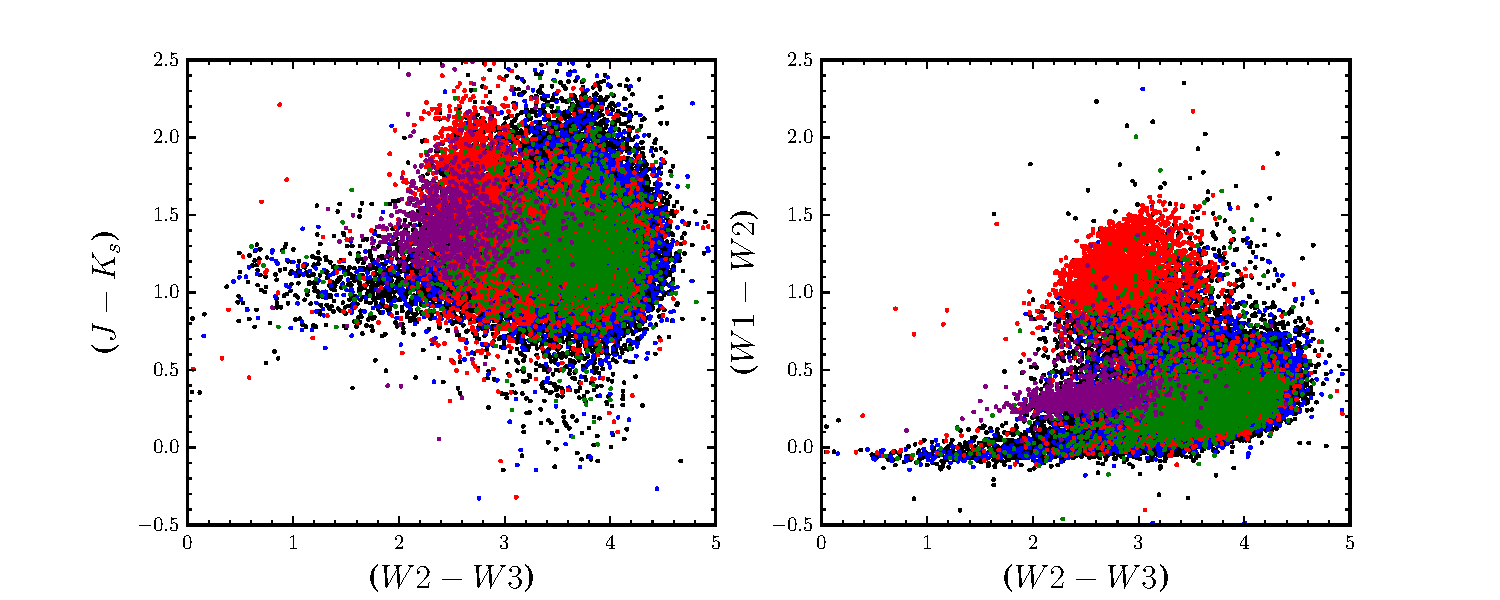
\includegraphics[width=6in]{figs/contaminant_color_color_distr.pdf}
\caption{Extragalactic sources from SDSS DR7's VAGC and LRG samples. Objects are (\emph{black}) starforming galaxies, (\emph{blue}) starburst galaxies, (\emph{red}) QSOs, (\emph{green}) AGN, and (\emph{purple}) LRGs. \label{fig:wisecontaminants}}
\end{figure}

\subsection{WISE+2MASS Young Stellar Objects}
Young Stellar Objects (YSOs) represent a unique contaminant in our search for dust-enshrouded AGB stars. Similar to AGBs, YSOs are luminous sources surrounded by warm, dusty environments. That warm dust can then glow brightly in the MIR, easily contaminating AGB color-color space. To characterize and later eliminate this potential contaminant, we select as our base sample 290 YSOs from \cite{2011ApJS..196....4R}, a survey searching for YSOs in the Taurus Molecular Cloud using data from WISE, ancillary data from SDSS and 2MASS, and covering 260 deg$^2$. As YSO tend to be embedded within high-extinction clouds, we expect that the dust-reddened NIR/MIR emission from these objects should match to similar objects in the LMC when we later calibrate our color-color criteria.

\subsection{WISE+2MASS Stellar Locus}
The color-color space occupied by AGB stars showing significant photospheric emission is heavily populated by naked stars from the main sequence. By sheer number, these stars would drown out sources that could be AGB stars with thin circumstellar envelopes. To address this, we extract the stellar locus from ALLWISE in the direction of the LMC ($276.5^\circ < l < 284^\circ$, $-38.2^\circ < b < -28^\circ$). We require that every object have 1 2MASS association, [$W1/W2/W3$] signal-to-noise $>$ 1, detections in 2MASS J, H, and K,  and confusion \& contamination flags set to 0 for [$W1/W2/W3$]. We then adapt the color-color criteria from \cite{2014MNRAS.440.3430D}. Their locus focuses on stars with effective temperatures $3540 < T_\text{eff} < 7200 K$. We fit their criteria for $J-K_s$ vs $W1 - W2$ within 3$\sigma$ of the locus with degree-3 polynomials. The resulting fit for the 3$\sigma$ stellar locus follows:

\begin{eqnarray}
(J - K_s) & < & 61.67(W1-W2)^3 - 17.88(W1-W2)^2 + 1.68(W1-W2) + 0.99\\
(J - K_s) & > & 40.19(W1-W2)^3 - 9.78(W1-W2)^2 + 0.54(W1-W2) + 0.64
\end{eqnarray}

The resulting locus sample, as well as the original \cite{2014MNRAS.440.3430D} bounds and locus are showin in Fig~\ref{fig:locus}. Note that our sample goes beyond the limits of the stated locus.

\begin{figure}[h]
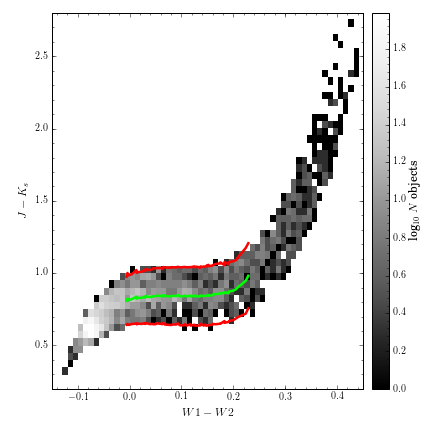
\includegraphics[width=3in]{figs/lmc_locus_3sig.png}
\caption{The WISE-2MASS stellar locus. (\emph{black dots}) objects from the stellar locus in the direction of the LMC. (\emph{blue line}) WISE-2MASS color-color stellar locus derived from \cite{2014MNRAS.440.3430D}. (\emph{red line}) 3$\sigma$ boundaries for WISE-2MASS color-color locus. \label{fig:locus}}
\end{figure}


\subsection{Merged Samples\label{sec:merged}}
The OGLE-III AGB sample, as well as the SDSS and YSO samples, were matched to the ALLWISE data products via the {\tt GATOR} tool at the NASA/IPAC Infrared Science Archive\footnote{\url{http://irsa.ipac.caltech.edu/cgi-bin/Gator/nph-scan?mission=irsa&submit=Select&projshort=WISE}}. The accepted matching radius was 3" execept in the case of YSOs, which were limited to 1". YSO objects were obtained from the VIZIER service already possessing WISE observations, so we were able to accept a smaller matching radius as we only sought the extra 2MASS information.

The final OGLE-2MASS-WISE AGB sample is produced from the obejct sample in section~\ref{sec:ogle}. We apply the point source saturation limits of [$W1/W2/W3/K_s$] $<$ [$2.0/1.5/-3.0/8.5$]. We also enforce, in order, the 5$\sigma$ faint limits for [$W1/W2/W3/K_s$]  $<$ [$16.83/15.6/11.32/15.5$]. The WISE point source saturation and 5$\sigma$ faint limits can be found in \cite{2012wise.rept....1C}. The 2MASS faint and saturation limits are found in \cite{2006AJ....131.1163S}. To ensure quality measurements in the desired bands, we also enforce [$W1/W2/W3$] SNR $> 3$, and contamination \& confusion flags ({\tt cc\_flag}) set to 0 in each of those bands. The VAGC, LRG, and YSO samples are filtered through the same criteria. Note that we deliberately neglect $W4$ because, after applying the 5$\sigma$ faint limits as well as {\tt cc\_flag}=0, our sample is too heavily reduced. The resulting populations from each reduction step can be found in Table~\ref{tab:reductions}.

\begin{table}[h]
	\begin{center}
	
	\scalebox{0.85}{

		\begin{tabular}{l r r r r r r r r r r}
		\hline\hline
		Population & OGLE & QSO & AGN & SF & SB & LRGs & YSOs & Locus & \textbf{Total} \\ 
		\hline
		Original & 46,262 & 122,550 & 19,184 & 232,845 & 67,128 & 105,631 & 290 & 25,254 & $\mathbf{619,267}$ \\
		WISE match & 43,209 & 6,902 & 3,098 & 36,539 & 10,359 & 75,543 & 274 & 25,254 & $\mathbf{201,178}$ \\
		$W1$-3, $K_s$ saturation limit& 43,201 & 6,900 & 3,098 & 36,538 & 10,358 & 75,527 & 214 & 25,156 & $\mathbf{200,992}$ \\
		 $W1$-2 faint limit & 43,200 & 6,891 & 3,098 & 36,537 & 10,358 & 75,527 & 214 & 24,382 & $\mathbf{200,207}$  \\
		 $W1$-3 faint limit & 19,358 & 6,728 & 3,005 & 35,678 & 10,105 & 1,184 & 214 & 3,154 & $\mathbf{79,426}$  \\
		 $W1$-3, $K_s$ faint limit & 19,358 & 5,283 & 2,878 & 34,299 & 9,676 & 1,167 & 213 & 3,070 & $\mathbf{75,944}$ \\
		 $W1$-3 SNR $> 3$ & 18,995 & 5,279 & 2,876 & 34,285 & 9,673 & 1,079 & 213 & 3,056 & $\mathbf{75,456}$\\
		\hline\hline
		\end{tabular}}    
	\caption{Sample populations with respect to each reduction step. Please see section~\ref{sec:merged} for the appropriate saturation limits, faint limits, and WISE matching radii.\label{tab:reductions}}
	\end{center}
	
\end{table}





%
%\subsection{XXX old stuff from here to the end of this section: Data Sources}
%\label{sec:sources}
%In this study, we rely heavily on data from the \allwise\, extension of the \wise\, survey, combining data from the initial All-Sky Data Release, the 3-band cryogenic data release, and the NEOWISE post-cryogenic data release \citep{2013wise.rept....1C}. The initial \wise\,All-Sky Data Release observed the sky between January and August 2010, observing the sky 1.2 times with four detectors, operating at 3.4, 4.6, 12, and 22$\mu$m. Hereon we refer to \allwise\, photometric bands at [3.4$\mu$m/4.6$\mu$m/12$\mu$m/22$\mu$m] as [$W1/W2/W3/W4$]. The positions of objects in the \wise\, catalog were calibrated to the \twomass\, point source catalog. The 3-band cryogenic data release contains data from $W1$, 2, and 3, and surveyed $30\%$ of the sky between August and October 2010. During the 3-band cryogenic survey, $W1$ and $W2$ operated with nearly the same sensitivity as during the full survey. Warming of the telescope reduced sensitivity in $W3$ and fully saturated $W4$. The NEOWISE post-cryogenic data release contains $W1$ and $W2$ measurements, with sensitivities close to those obtained during the full cryogenic phase. During this phase, \wise\, surveyed $70\%$ of the sky. Data products from the post-cryogenic release included updated instrumental, astrometric, and photometric calibrations and reduction algorithms, resulting in much lower SNR. The overall number of sources compiled into \allwise\, totals over 747.6 million.
%
%In order to generate a reliable, high-confidence catalog of Galactic candidate \agb\, stars, we must first define color-color criteria from known \agb\, star samples. We select \agb\, stars from three source catalogs: the {\it Optical Gravitational Lens Experiment-III Variable Star Catalog} \citep[\ogle,][]{2008AcA....58...69U,2009AcA....59..239S,2011AcA....61..217S}, the {\it MAssive Compact Halo Objects} project \citep[\macho,][]{1997ApJ...482...89A}, and the \simbad\, Astronomical Database \citep{2000A&AS..143....9W}. 
%
%\ogle\, photometry for Long-Period Variables (LPVs) in the Small and Large Magellanic Clouds (SMC and LMC respsectively) was obtained between July 2001 and May 2009, with stars in the central 4.5-deg$^2$ of the LMC and SMC having an additional 5 observing seasons of photometry from OGLE-II. LPVs were classified into 3 categories: \ogle\, Small Amplitude Red Giants (OSARGs), Semi-Regular Variables (SRVs), and Miras. All AGB stars  O-rich and C-rich \agb\, stars in \ogle\, were photometrically selected using reddening-free Wesenheit magnitudes, described in detail in \cite{2009AcA....59..239S,2011AcA....61..217S}. {\color{red}[Describe the selection bit in a little more detail, along with their sample completeness, selection biases, and contamination fractions]} Data reduction techniques are described in \cite{2008AcA....58...69U}. The resulting samples yield 46,467 \agb\, stars from the LMC (37,203 O-rich; 9,264 C-rich) and 6,509 stars from the SMC (3,727 O-rich; 2,782 C-rich). 
%
%From \macho\, we obtain the sample of SMC, LMC, and Galactic Bulge AGB stars used in \cite{2008AJ....136.1242F} (14,861 stars). {\color{red}Why were these objects selected? Howe were they selected? What is their completeness, selection bias, and contamination fraction?} Following \cite{2008AJ....136.1242F}, the objects are divided into sequences (seq) 1-4. Sequence 1 primarily contains Mira variables pulsating in their fundamental modes, whereas Sequences 2-4 contain semi-regular variables in various pulsation modes.
%
%The sample of AGB stars from \simbad\, was obtained by querying all objects classified as C-stars (18,656), S-stars (1,108), OH/IR stars (825), AGB stars (2,359), and Mira variables (9,608), for a total of 32,556 stars. Objects are classified spectroscopically, though by a variety of methods owing to the heterogeneous data housed within \simbad. Together with \macho\, and \ogle, the total sample of \agb\, stars is 100,393. Because there is a high likelihood that samples between \ogle, \macho, and \simbad overlap, we retain only unique objects after the initial data reduction in section~\ref{sec:reduction}.
%
%We use \sdss\, spectroscopic catalogs to find and quantify regions in NIR-MIR color-color space populated by plausible contaminant sources. These include any Galactic stellar objects and planetary nebulae, as well as a host of extragalactic sources. Data for active galactic nuclei (AGN; 19,184 objects), quasi-stellar objects (QSOs; 122,550 objects), and star forming/burst galaxies (820,272 objects total) were drawn from \sdss\, DR7, specifically from the NYU Value Added Galaxy Catalog\footnote{\url{http://sdss.physics.nyu.edu/vagc/}} \citep[VAGC]{2005AJ....129.2562B}. Luminous Red Galaxies (LRGs) were selected from the SDSS Luminous Red Galaxy Survey \citep[105,631 objects, ][]{2010ApJ...710.1444K}.  Data for stars in the SDSS stellar locus were drawn from the DR 9 SEGUE Stellar Parameters Pipeline (SSPP) \citep[1,843,190 objects, ][]{2012ApJS..203...21A}. {\color{red} Include bit about YSOs and PNe from SIMBAD}
%
%\subsection{Data Reduction}
%\label{sec:reduction}
%We use NASA/IPAC IRSA's {\tt GATOR} tool\footnote{\url{http://irsa.ipac.caltech.edu/cgi-bin/Gator/nph-scan?mission=irsa&submit=Select&projshort=WISE}} to positionally match \sdss, \ogle, \macho, and \simbad\, to \allwise. We select only matches within 3" between  each sample and \allwise. All samples of \agb\, were required to be brighter than the published 5$\sigma$ faint limits of [16.83/15.6/11.32/8.0], as well as fainter than the saturation limits of [2.0/1.5/-3.0/-4.0] extrapolated from the wings of the PSFs for point sources, for [$W1/W2/W3/W4$] \citep{2013wise.rept....1C}, with no flags for confusion or contamination as a spurious source in any band. We also require only single associations with \twomass\, objects within 3", detections in [$J/K_s/W1/W2/W3/W4$], and SNR $>$ 3 in each \allwise\, band. 
%
%The population for each sample from initial matching as well as after the application of the \allwise\, faint limits, saturation limits, and \twomass\, detection requirements are shown in Table~\ref{tab:pop}. The WISE color-color distributions for the AGB and contaminant samples are shown in Figure~\ref{fig:distros}. \\
%
%\vspace{-10pt}
%%\begin{table}[h]
%%	\begin{center}
%%	\caption{AGB and Contaminant Populations}
%%	\scalebox{0.85}{\begin{tabular}{l c c c c c c}
%%		\hline
%%		Population & SIMBAD C stars & OH/IR stars & Miras & S stars & AGB stars \\
%%		\hline
%%		2" match & 13,245 & 294 & 8,850 & 1,078 & 1,665 \\
%%		Reduced & 3,327 & 165 & 6,218 & 865 & 1,121 \\
%%		\hline\hline
%%		Population & MACHO seq1 & seq2 & seq3 & seq4\\
%%		\hline
%%		2" match & 5,193 & 3,441 & 2,548 & 2,931 \\
%%		Reduced & 927 & 642 & 263 & 336 \\
%%		\hline\hline
%%		Population & OGLE C-rich & O-rich\\
%%		\hline
%%		2" match & 11,417 & 38,369 \\
%%		Reduced & 737 & 2515 \\
%%		\hline\hline
%%		Population & Locus Stars & AGN & LRG & QSO & Galaxies \\
%%		\hline
%%		2" match & 1,508,158 & 18,481 & 102,178 &  & 799,761 \\
%%		Reduced & 168,045 & 9,652 & 7,717 & 18,360 & 125,869 \\
%%		\hline
%%
%%		\label{tab:pop}
%%	\end{tabular}}
%%	\end{center}
%%\end{table}
%
%\begin{table}[h]
%	\begin{center}
%	
%	\scalebox{0.85}{\begin{tabular}{l c c c c c c}
%		\hline\hline
%		Population & SIMBAD AGB* & C* & Mira & OH/IR & S* \\ 
%		\hline
%		3" match & 1,689 & 14,209 & 9,027 & 406 & 1,081 \\
%		Reduced & 684 & 1,782 & 3,241 & 43 & 511 \\ 
%		\hline
%		Population & MACHO seq1 & seq2 & seq3 & seq4 \\ 
%		\hline
%		3" match & 5,279 & 3,519 & 2,619 & 3,070 \\
%		Reduced & 277 & 185 & 73 & 61 \\ 
%		\hline
%		Population & OGLE-III C-rich & O-rich \\ 
%		\hline
%		3" match & 11,542 & 38,848 \\
%		Reduced & 249 & 730 \\ 
%		\hline
%		Population & DR12 SSPP & DR7 LRG & QSO & AGN & Galaxies \\ 
%		\hline
%		3" match & 1,578,329 & 104,345 & 103,590 & 18,528 & 841,712 \\ 
%		Reduced & 67,508 & 84 & 3,977 & 1,069 & 44,314 \\ 
%		\hline\hline
%
%		
%	\end{tabular}}    
%	\caption{\agb\, and contaminant populations matched to WISE before and after sample reduction in section~\ref{sec:reduction}. MACHO sequences (seq1-seq4) are from \cite{2008AJ....136.1242F} and described briefly in section~\ref{sec:sources}.\label{tab:pop}}
%	\end{center}
%	
%\end{table}
%
%\begin{figure}
%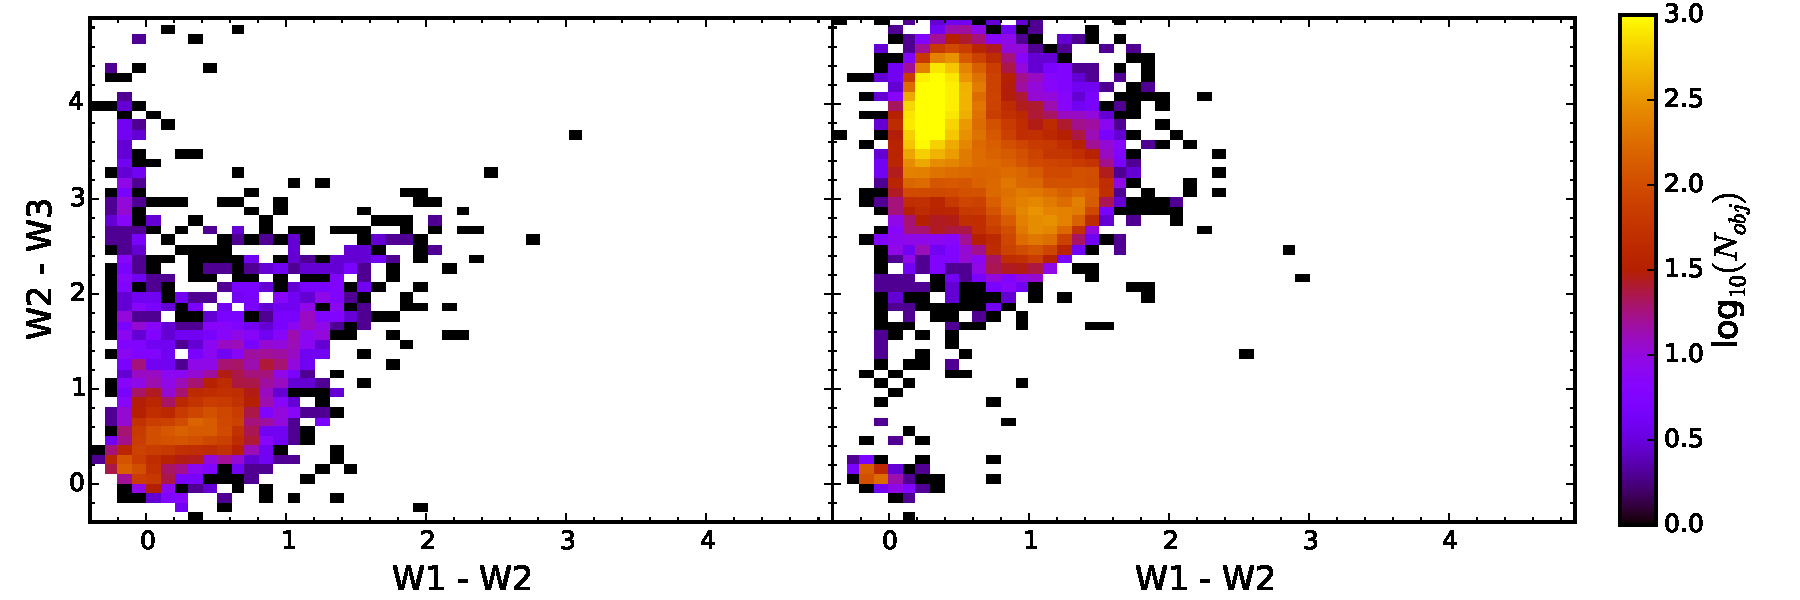
\includegraphics[width=7in]{figs/agbs_contaminants_color_color1.pdf}
%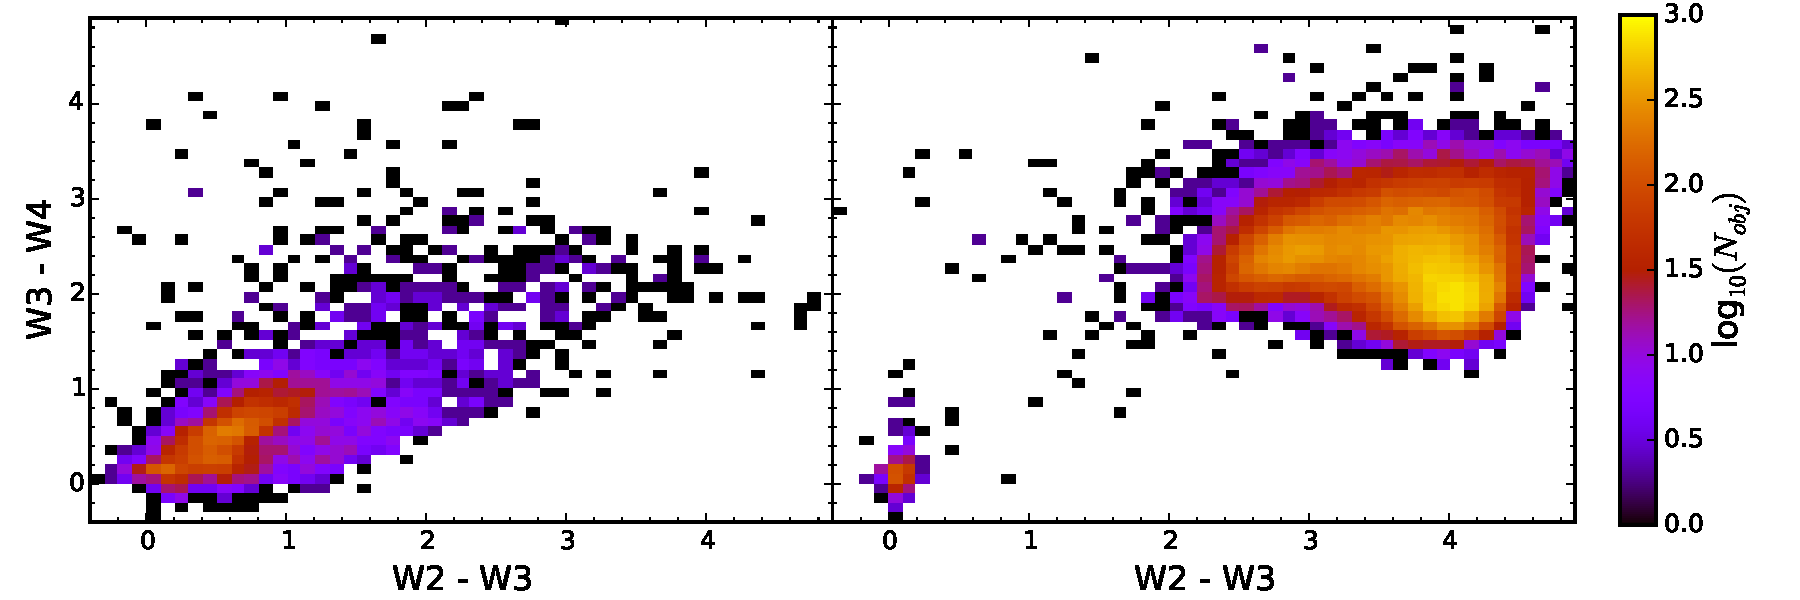
\includegraphics[width=7in]{figs/agbs_contaminants_color_color2.pdf}
%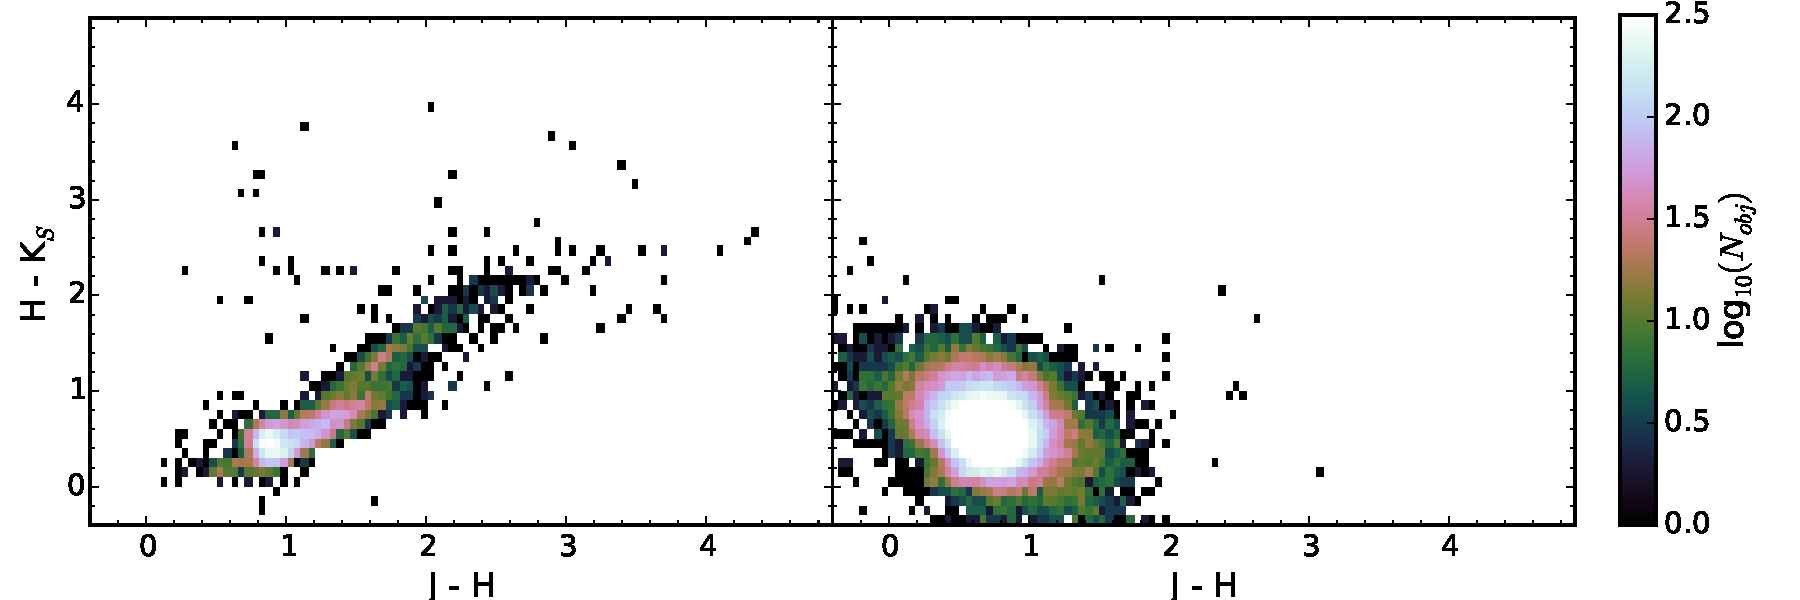
\includegraphics[width=7in]{figs/agbs_contaminants_color_color3.pdf}
%\caption{Logarithmic number densities for objects in \wise\, and \twomass\, color-color space, binned in 0.1 dex on each axis. \emph{Left:} The combined AGB sample matched to ALLWISE. \emph{Right:} The combined contaminant sample.\label{fig:distros}}
%\end{figure}

